\chapter{SİSTEM MİMARİSİ}

Aura Finance, modern finansal takip ve yapay zekâ tabanlı bütçe optimizasyonu sunan bir web uygulamasıdır. Bu bölümde, sistemin genel yapısı, kullanılan teknolojiler ve veri modelleri detaylandırılmıştır.

\section{Genel Sistem Mimarisi}

Sistem, monorepo yapısında tasarlanmış olup üç ana katmandan (three-tier architecture) oluşmaktadır:
\begin{enumerate}
    \item \textbf{İstemci Katmanı (Frontend):} React (Vite) ve TypeScript kullanılarak geliştirilen kullanıcı arayüzü.
    \item \textbf{Uygulama Katmanı (Backend):} Node.js ve Express.js tabanlı API servisleri.
    \item \textbf{Yapay Zekâ Katmanı (AI Layer):} TensorFlow.js ve Python tabanlı modelleri içeren hibrit yapı.
\end{enumerate}

Şekil~\ref{fig:mimari_diyagram} sistemin genel çalışma prensibini ve katmanlar arası etkileşimi göstermektedir.

\begin{figure}[h!]
 \centering
 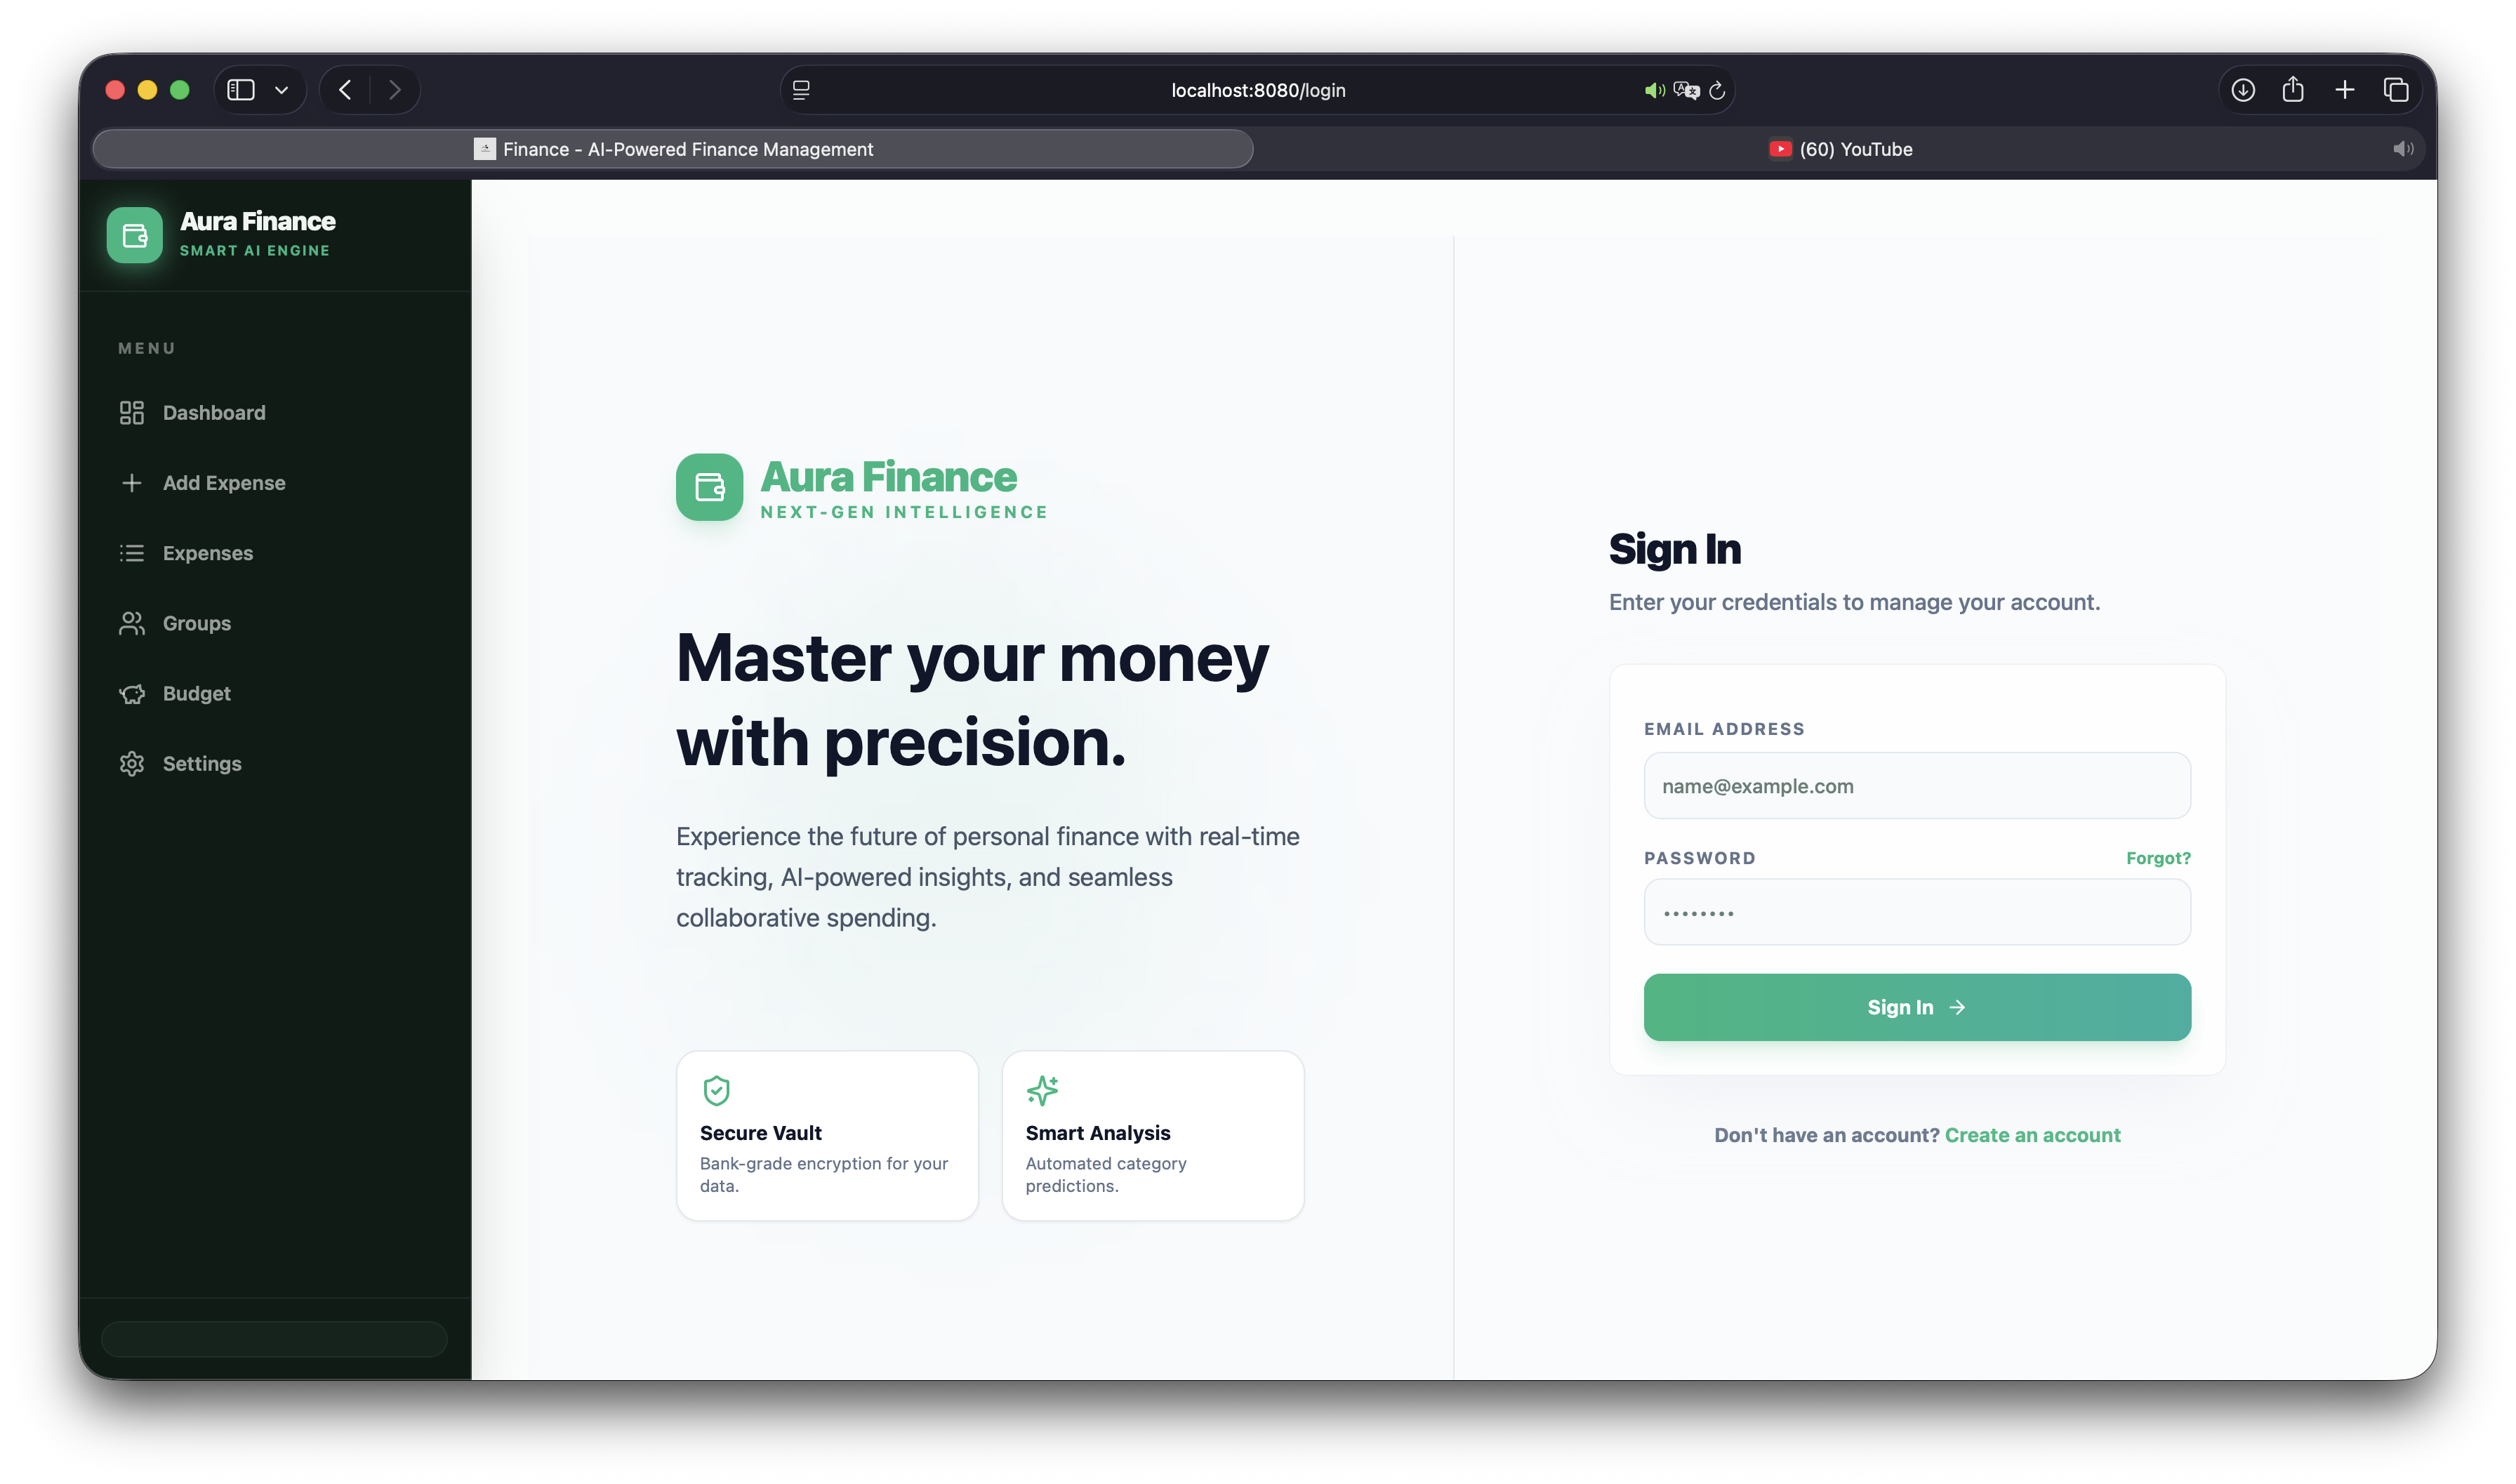
\includegraphics[width=0.8\textwidth]{./fig/aura_sc1} % Placeholder for architecture diagram if available
 \caption{Aura Finance Genel Sistem Mimarisi ve Katmanlı Yapı.}
 \label{fig:mimari_diyagram}
\end{figure}

\section{İstek-Yanıt Döngüsü ve Güvenlik}

Sistemdeki tüm veri trafiği JWT (JSON Web Token) tabanlı kimlik doğrulama ile korunmaktadır. Kullanıcı sisteme giriş yaptığında sunucu tarafından bir token üretilir ve sonraki tüm isteklerde bu token "Authorization" başlığında iletilir. Sunucu, gelen isteği doğrular ve yetki seviyesine göre veritabanı veya AI servislerine erişim sağlar.

\section{Veritabanı Varlık-İlişki Diyagramı (ERD)}

Sistemin kalbinde PostgreSQL veritabanı yer almaktadır. Veri modelleri Prisma ORM kullanılarak yönetilmiştir. Temel tablolar ve ilişkileri aşağıda açıklanmıştır:

\begin{itemize}
    \item \textbf{User (Kullanıcı):} Kimlik bilgileri ve aylık gelir verisi.
    \item \textbf{Expense (Harcama):} Tutar, tarih, kategori ve grup ilişkisi.
    \item \textbf{Budget (Bütçe):} Kategori bazlı limitler.
    \item \textbf{Category (Kategori):} Sabit harcama kategorileri (Gıda, Ulaşım, vb.).
\end{itemize}

Şekil~\ref{fig:erd_diyagram} veritabanı şemasını ve tablolar arası ilişkileri temsil etmektedir.

\begin{figure}[h!]
 \centering
 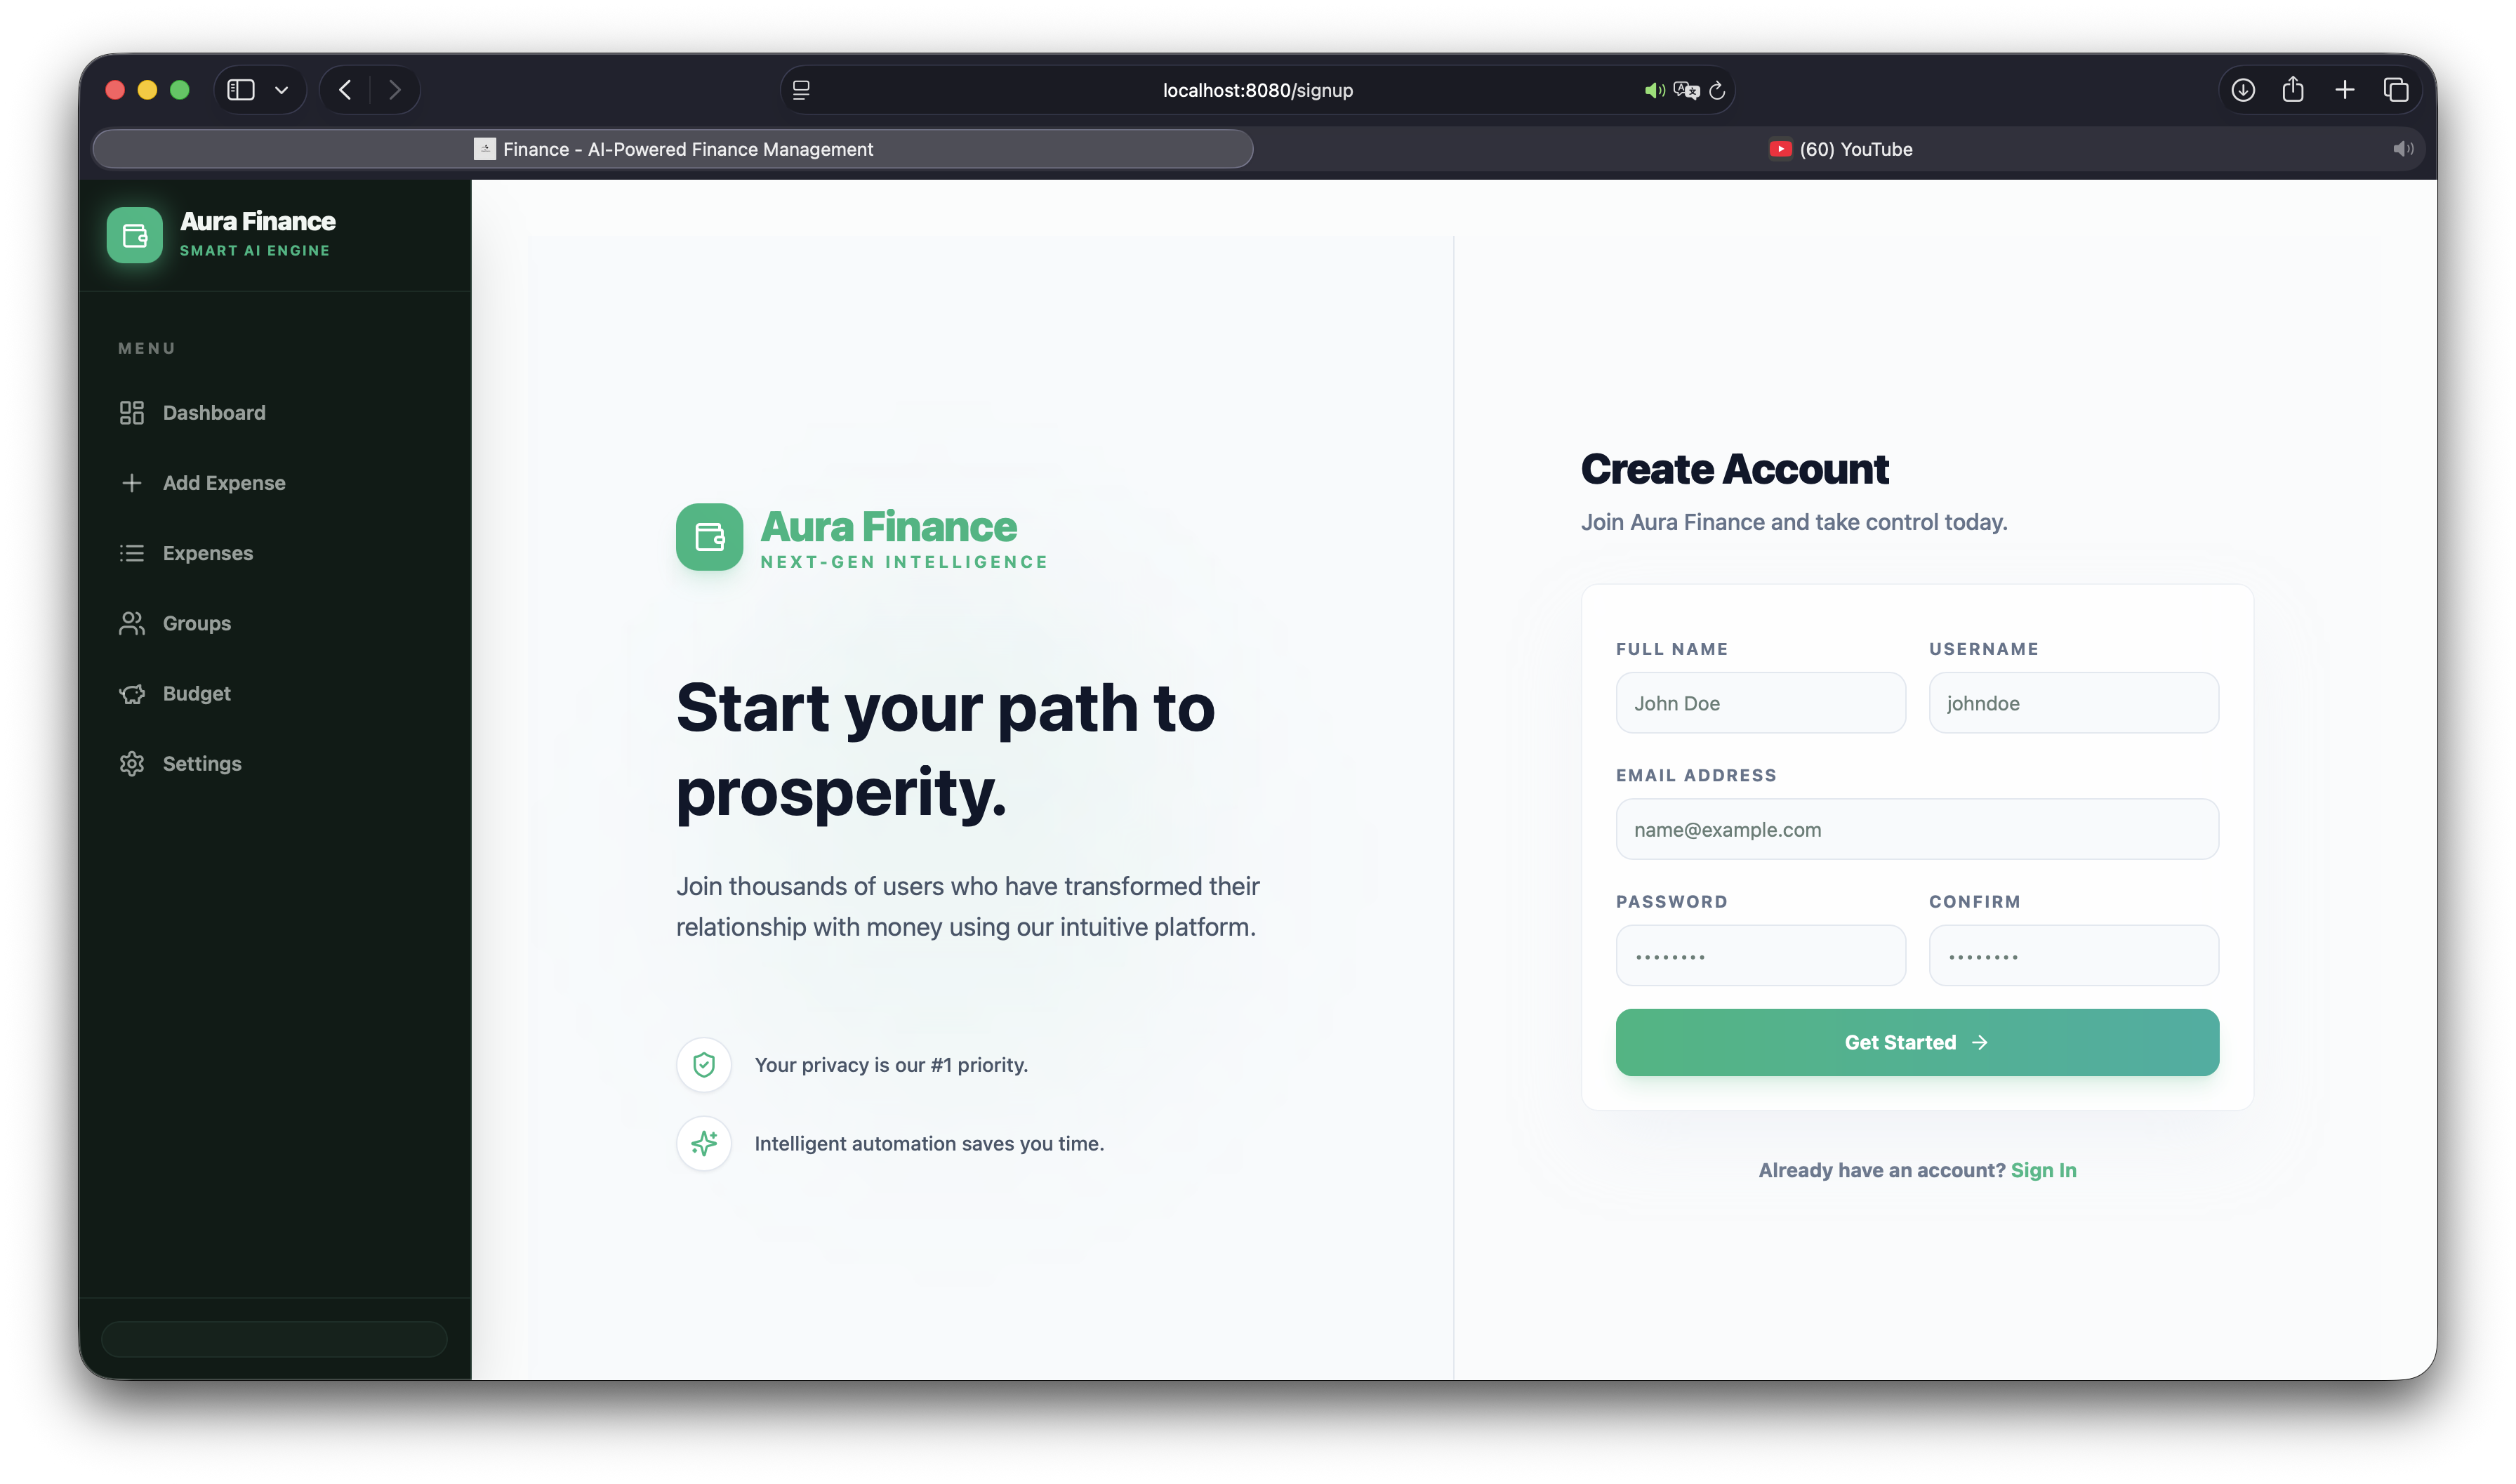
\includegraphics[width=0.7\textwidth]{./fig/aura_sc2} % Placeholder for ERD
 \caption{Veritabanı Varlık-İlişki Diyagramı (ERD).}
 \label{fig:erd_diyagram}
\end{figure}

\section{Teknoloji Yığını}

Aura Finance, yüksek performans ve tip güvenliği için \textbf{TypeScript} ile yazılmış bir \textbf{React} uygulamasıdır. Sunucu tarafında \textbf{Node.js} ve \textbf{Express.js} kullanılmış, veritabanı işlemleri için \textbf{Prisma} tercih edilmiştir. Yapay zekâ modülleri ise \textbf{TensorFlow.js} ve \textbf{XGBoost} ile hibrit bir yapıda kurgulanmıştır.
